\section{Tiền xử lý và Khám phá dữ liệu (EDA)}

\subsection{Khám phá dữ liệu thô (Raw Data EDA)}
Trước khi tiến hành bất kỳ thao tác xử lý nào, nhóm thực hiện khảo sát trạng thái nguyên bản của tập dữ liệu \textbf{water\_potability.csv} để nhận diện các vấn đề về chất lượng dữ liệu.

\subsubsection{Tổng quan cấu trúc}
Bộ dữ liệu bao gồm 3.276 bản ghi với 10 đặc trưng hóa lý. Qua quan sát sơ bộ bằng lệnh \texttt{df.head()}, dữ liệu thô xuất hiện nhiều giá trị \textbf{NaN} (Not a Number) tại các cột quan trọng.

\subsubsection{Phân tích dữ liệu thiếu (Missing Values)}
Đây là vấn đề nghiêm trọng nhất của bộ dữ liệu này. Nhóm thực hiện thống kê số lượng dòng thiếu trên từng thuộc tính:

\begin{figure}[H]
    \centering
    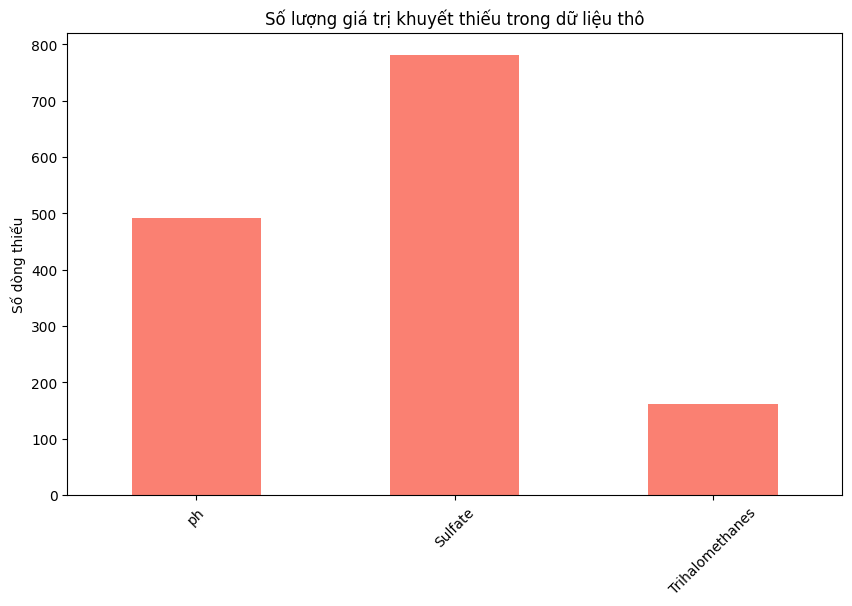
\includegraphics[width=0.7\textwidth]{IMAGE/raw_missing.png}
    \caption{Thống kê các cột bị khuyết thiếu dữ liệu trong tập thô}
    \label{fig:raw_missing}
\end{figure}

\textbf{Nhận xét:} Cột \textbf{Sulfate} bị khuyết nhiều nhất với hơn 700 dòng, tiếp đến là \textbf{ph} và \textbf{Trihalomethanes}. Nếu thực hiện xóa bỏ các dòng này, nhóm sẽ mất đi khoảng 30\% lượng dữ liệu huấn luyện, gây ảnh hưởng đến độ chính xác của mô hình AI.

\subsection{Quy trình Tiền xử lý dữ liệu (Data Preprocessing)}
Dựa trên các vấn đề đã nhận diện tại bước EDA thô, nhóm tiến hành xây dựng quy trình ETL (Extract - Transform - Load) tự động. Mục tiêu của quy trình này không chỉ là làm sạch dữ liệu mà còn tái cấu trúc thông tin để phù hợp với kiến trúc kho dữ liệu Star Schema.

\subsubsection{Làm sạch dữ liệu (Data Cleaning)}
Nhóm nhận diện có 3 thuộc tính quan trọng bị khuyết thiếu dữ liệu diện rộng: pH (491 dòng), Sulfate (781 dòng) và Trihalomethanes (162 dòng). Để bảo toàn dung lượng mẫu cho việc huấn luyện AI mà không làm thay đổi đặc tính thống kê chung, nhóm áp dụng phương pháp \textbf{Mean Imputation} (điền khuyết bằng giá trị trung bình) thông qua bước xử lý \texttt{If field value is null} trong Pentaho.

Các tham số cụ thể được thiết lập dựa trên giá trị trung bình tính toán từ tập mẫu sạch:
\begin{itemize}
    \item \textbf{Cột pH:} Điền giá trị $7.08$.
    \item \textbf{Cột Sulfate:} Điền giá trị $333.77$.
    \item \textbf{Cột Trihalomethanes:} Điền giá trị $66.39$.
\end{itemize}

\subsubsection{Kỹ thuật Đặc trưng và Phân nhóm (Feature Engineering - Binning)}
Đây là giai đoạn quan trọng nhất để chuyển đổi dữ liệu từ dạng số liên tục sang dạng danh mục, phục vụ cho việc phân tích đa chiều trong kho dữ liệu. Nhóm sử dụng bước \texttt{Number range} để phân loại các chỉ số dựa trên các tiêu chuẩn hóa lý:

\begin{itemize}
    \item \textbf{Phân loại nồng độ pH (Dim\_Acidity):}
    \begin{itemize}
        \item \textbf{Axit:} pH $< 6.5$.
        \item \textbf{Trung tính:} $6.5 \le \text{pH} \le 8.5$.
        \item \textbf{Kiềm:} pH $> 8.5$.
    \end{itemize}
    \item \textbf{Phân loại độ cứng (Dim\_Hardness):}
    \begin{itemize}
        \item \textbf{Nước mềm:} Hardness $< 60$ mg/L.
        \item \textbf{Nước cứng vừa:} $60 \le \text{Hardness} < 120$ mg/L.
        \item \textbf{Nước cứng:} $120 \le \text{Hardness} < 180$ mg/L.
        \item \textbf{Nước rất cứng:} Hardness $\ge 180$ mg/L.
    \end{itemize}
\end{itemize}

% \subsubsection{Hiện thực hóa quy trình ETL bằng Pentaho Data Integration}
% Để tự động hóa việc luân chuyển dữ liệu từ tập tin thô vào kho dữ liệu, nhóm sử dụng công cụ \textbf{Pentaho Data Integration (PDI)}. Toàn bộ logic tiền xử lý, biến đổi đặc trưng và quản lý khóa thay thế (Surrogate Keys) được đóng gói trong tệp luồng xử lý \texttt{water\_etl\_pipeline.ktr}.

% Quy trình xử lý dữ liệu trong Pentaho được thiết kế theo trình tự tuyến tính để đảm bảo tính toàn vẹn của dữ liệu qua từng bước:

% \begin{itemize}
%     \item \textbf{Dữ liệu đầu vào:} Trích xuất từ tệp CSV gốc thông qua step \texttt{CSV file input}.
%     \item \textbf{Xử lý giá trị khuyết thiếu:} Nhóm sử dụng step \texttt{If field value is null} để điền các giá trị trung bình đã tính toán: pH ($7.08$), Sulfate ($333.77$) và Trihalomethanes ($66.39$).
%     \item \textbf{Phân loại và Rời rạc hóa:} Các step \texttt{Number range} thực hiện logic chia ngưỡng cho độ pH và độ cứng của nước để tạo ra các danh mục đặc trưng.
%     \item \textbf{Quản lý bảng Dimension:} Sử dụng \texttt{Combination lookup/update} để sinh khóa Surrogate Key tự động, đảm bảo kho dữ liệu hoạt động ổn định và tối ưu hiệu suất truy vấn.
%     \item \textbf{Nạp dữ liệu vào bảng Fact:} Kết thúc bằng step \texttt{Table output} để nạp toàn bộ dữ liệu sạch vào bảng \texttt{Fact\_Water\_Sample} trong cơ sở dữ liệu.
% \end{itemize}

% \begin{figure}[H]
%     \centering
%     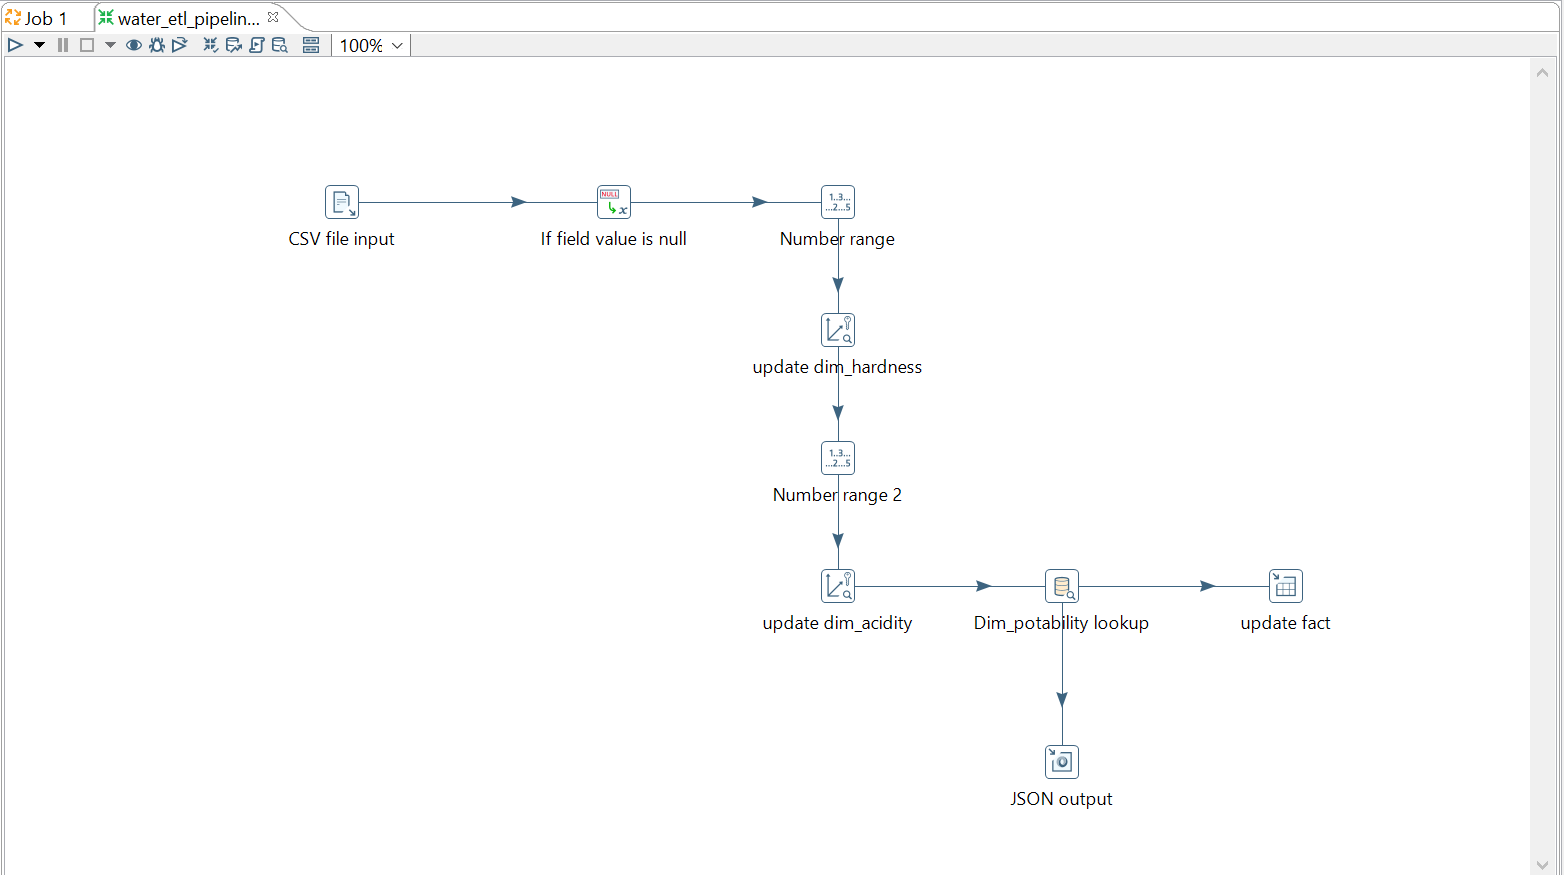
\includegraphics[width=1\textwidth]{IMAGE/pentaho_flow.png} 
%     \caption{Sơ đồ luồng xử lý dữ liệu tự động trong giao diện Pentaho}
%     \label{fig:pentaho_flow}
% \end{figure}

\subsection{Khám phá dữ liệu sau tiền xử lý (Clean Data EDA)}
Sau khi hoàn tất quy trình làm sạch và điền khuyết tại Mục 3.2, nhóm tiến hành phân tích chi tiết toàn bộ các chỉ số hóa lý. Đây là bước quan trọng để xác nhận dữ liệu đã sẵn sàng cho việc huấn luyện mô hình và xây dựng kho dữ liệu.

\subsubsection{Phân tích mối quan hệ đa biến (Correlation Matrix)}
Nhóm sử dụng ma trận tương quan để đánh giá lại mối liên hệ giữa các thuộc tính sau khi đã xử lý dữ liệu thiếu.

\begin{figure}[H]
    \centering
    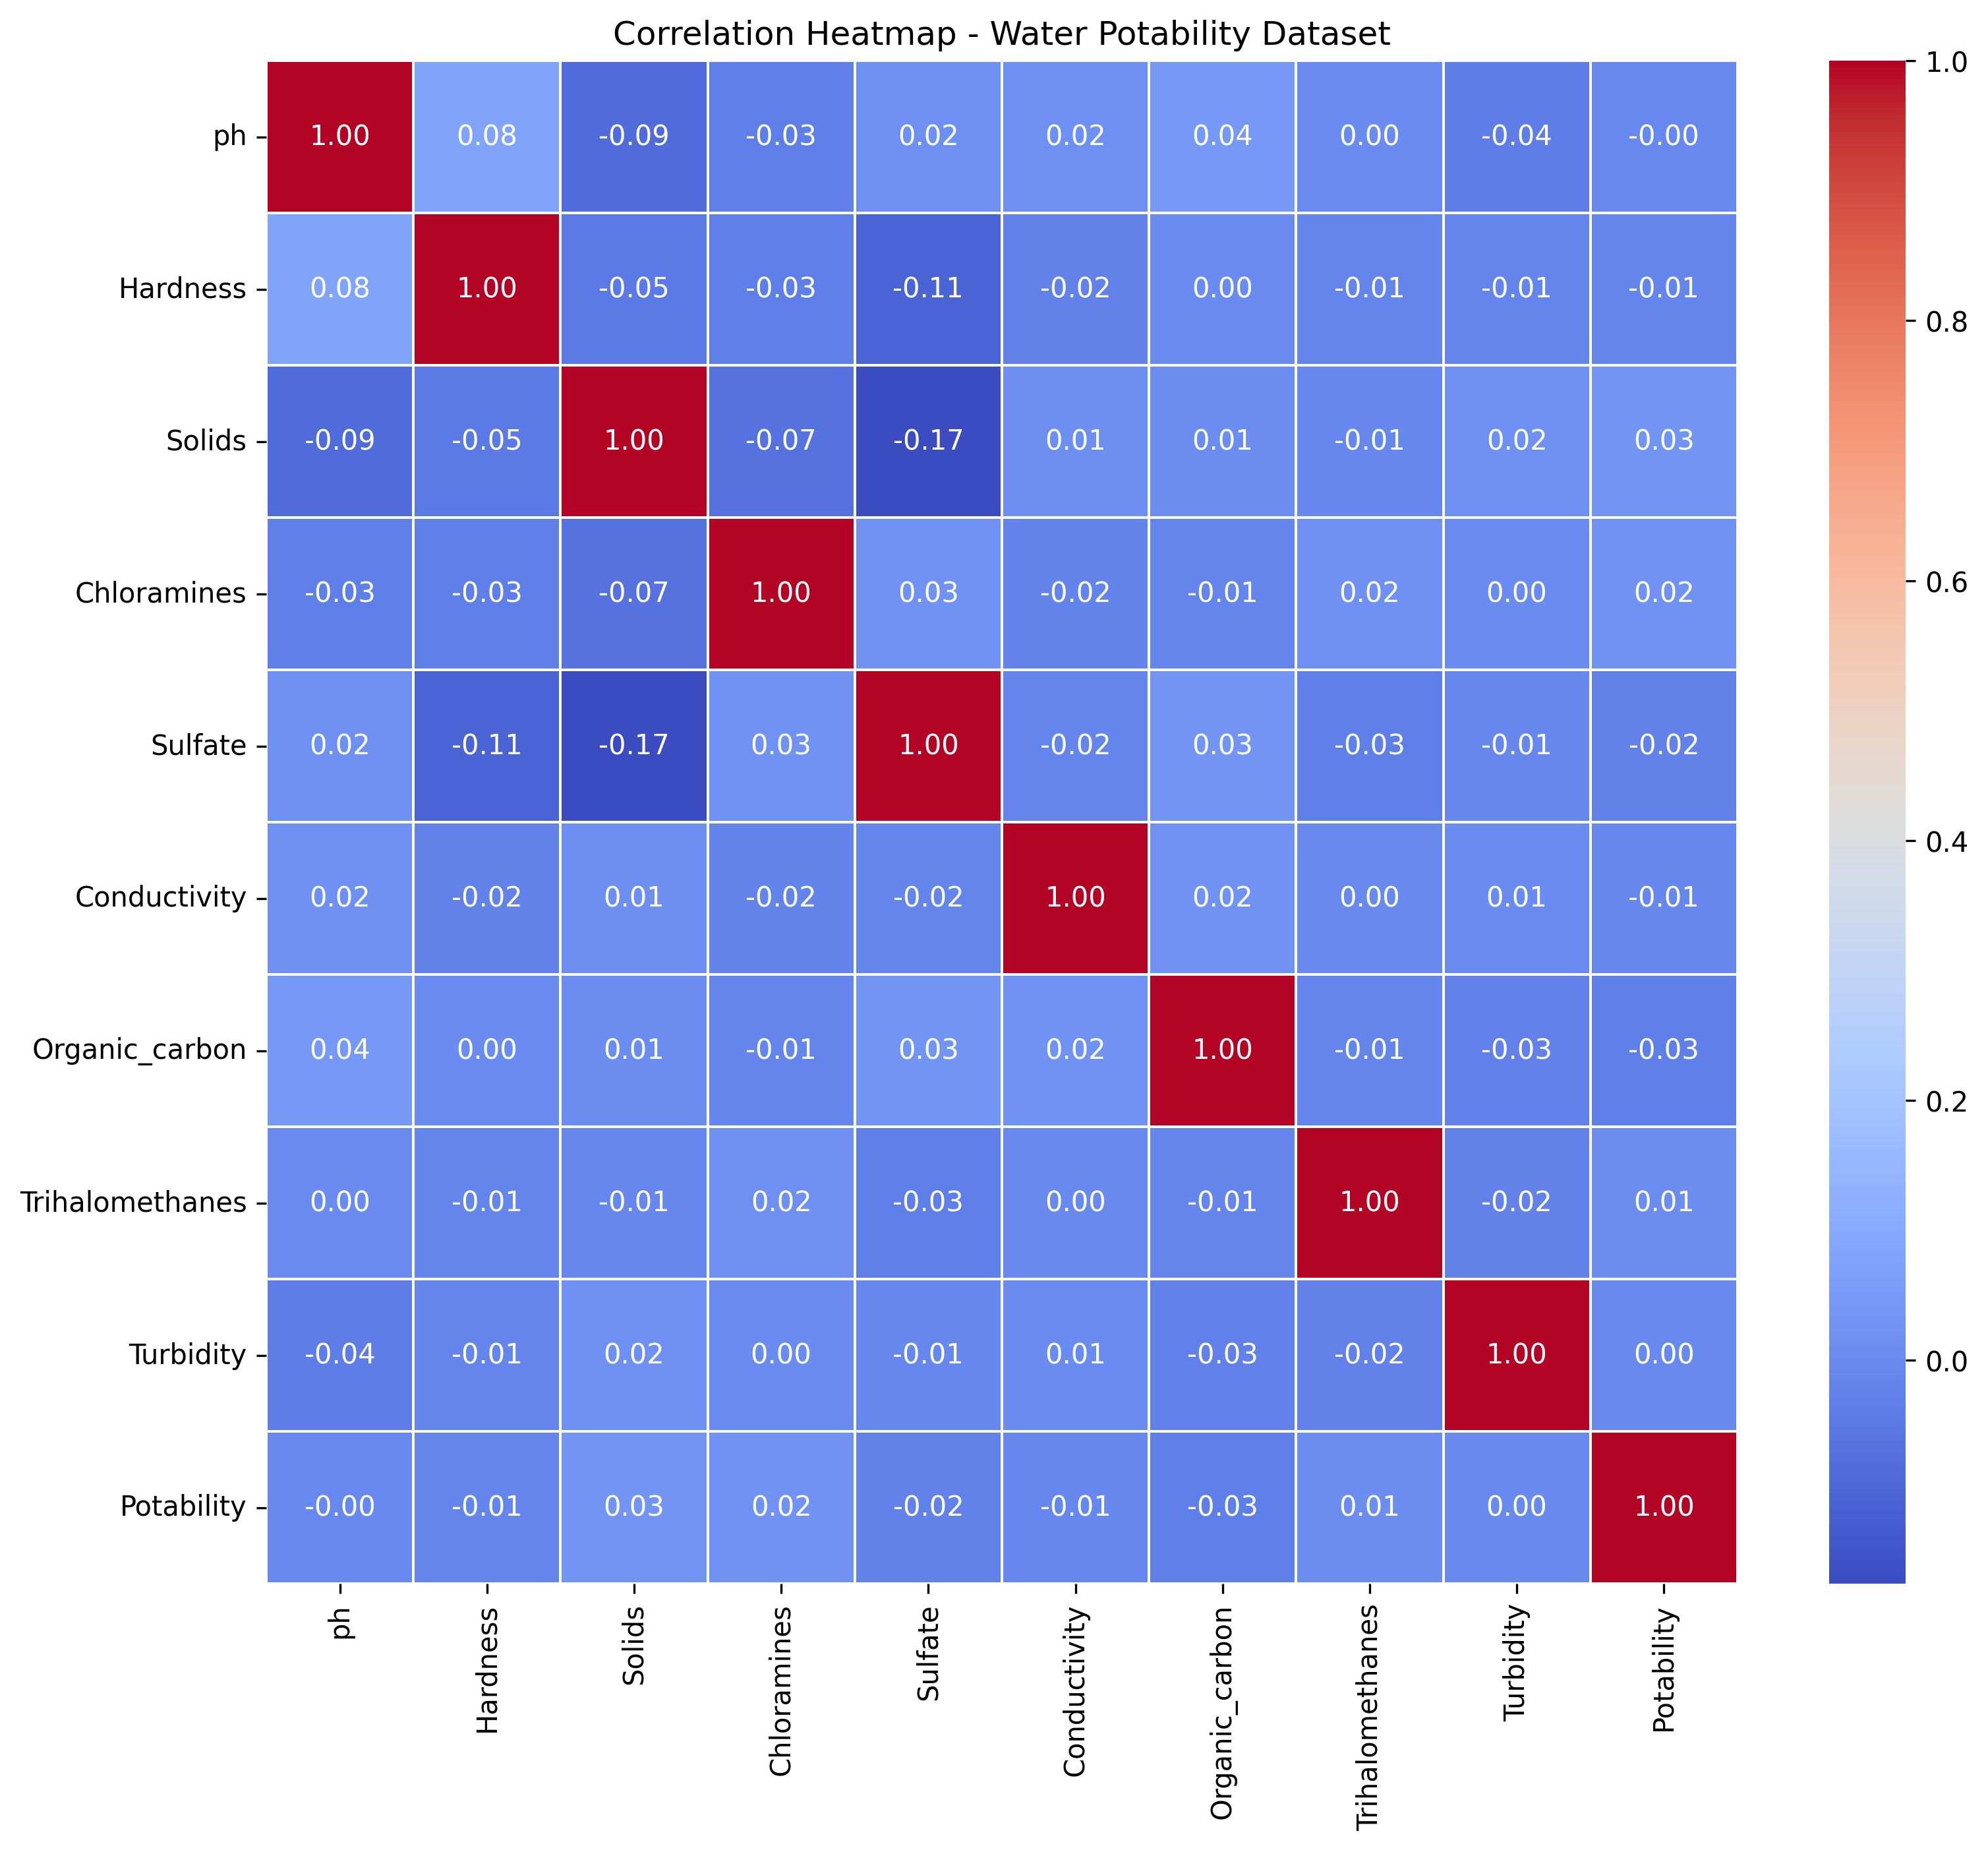
\includegraphics[width=0.8\textwidth]{IMAGE/heatmap.png}
    \caption{Ma trận tương quan của dữ liệu sau tiền xử lý}
\end{figure}

\textbf{Nhận xét:} Hầu hết các đặc trưng (pH, Hardness, Sulfate,...) đều có tương quan xấp xỉ bằng $0$ với nhãn Potability. Điều này minh chứng cho tính độc lập cao giữa các đặc trưng, tránh hiện tượng đa cộng tuyến và tạo điều kiện thuận lợi cho các thuật toán phi tuyến tính.

\subsubsection{Phân tích các biến rời rạc (Categorical Analysis)}
Sau khi thực hiện kỹ thuật Binning trong quy trình ETL để tạo ra các nhóm phân loại mới, nhóm tiến hành so sánh tỉ lệ an toàn (Potability) giữa các danh mục này để tìm kiếm các đặc điểm đặc trưng của nguồn nước an toàn.

\begin{figure}[H]
    \centering
    \begin{minipage}{0.48\textwidth}
        \centering
        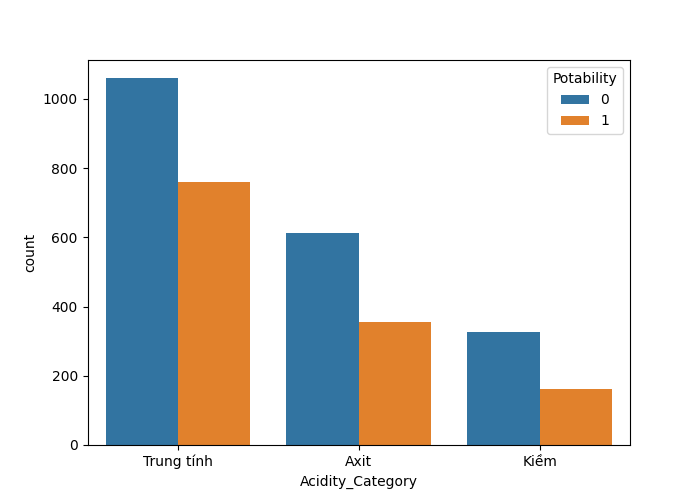
\includegraphics[width=1\textwidth]{IMAGE/discrete_acidity.png}
        \caption{Tỉ lệ Potability theo nồng độ pH (Dim\_Acidity)}
    \end{minipage}
    \hfill
    \begin{minipage}{0.48\textwidth}
        \centering
        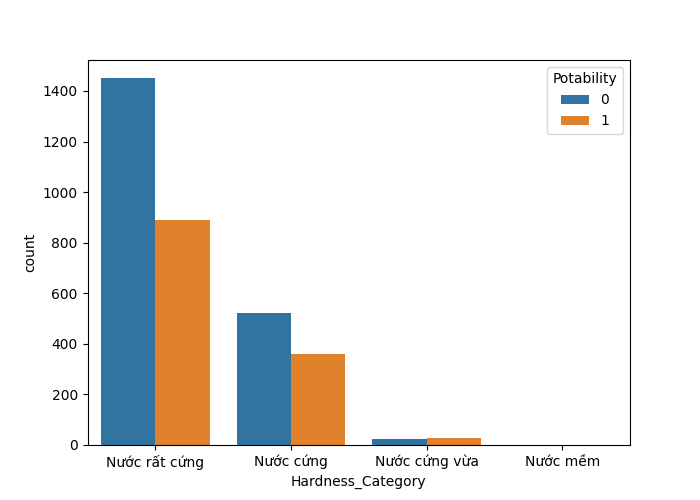
\includegraphics[width=1\textwidth]{IMAGE/discrete_hardness.png}
        \caption{Tỉ lệ Potability theo độ cứng (Dim\_Hardness)}
    \end{minipage}
\end{figure}

Qua các biểu đồ thống kê trên, nhóm rút ra các kết luận quan trọng phục vụ cho việc phân tích chất lượng nước:
\begin{itemize}
    \item \textbf{Về nồng độ pH (Acidity\_Category):} 
    \begin{itemize}
        \item Nhóm nước \textbf{Trung tính} chiếm tỷ trọng áp đảo với hơn 1.000 mẫu không an toàn và gần 800 mẫu an toàn. 
        \item Tiếp theo là nhóm nước \textbf{Axit} và cuối cùng là nhóm nước \textbf{Kiềm}. 
        \item Tỷ lệ giữa nước uống được (Potability = 1) và không uống được (Potability = 0) duy trì khá đồng nhất trên cả 3 phân loại, cho thấy tính axit hay kiềm đơn lẻ không phải là yếu tố quyết định sự khác biệt lớn về độ an toàn.
    \end{itemize}
    
    \item \textbf{Về độ cứng (Hardness\_Category):}
    \begin{itemize}
        \item Tập dữ liệu cho thấy một sự tập trung cực kỳ lớn vào nhóm \textbf{Nước rất cứng} (vượt mốc 1.400 mẫu ở nhãn 0).
        \item Nhóm \textbf{Nước cứng} đứng vị trí thứ hai với tổng số lượng mẫu đáng kể, trong khi nhóm \textbf{Nước cứng vừa} chiếm tỷ lệ rất thấp.
        \item Đặc biệt, nhóm \textbf{Nước mềm} gần như không xuất hiện hoặc chiếm số lượng không đáng kể trong tập dữ liệu này.
        \item Tương tự như pH, phân phối của nhãn Potability trên các nhóm độ cứng không có sự chênh lệch đột biến, củng cố giả thuyết về mối quan hệ phi tuyến tính phức tạp giữa các biến.
    \end{itemize}
\end{itemize}

\subsubsection{Phân tích chi tiết các biến liên tục}
Nhóm thực hiện trực quan hóa phân phối cho từng biến để kiểm chứng tác động của quy trình ETL và nhận diện đặc tính dữ liệu sạch.

\paragraph{Biến "ph":} \leavevmode\\
\begin{figure}[H]
    \centering
    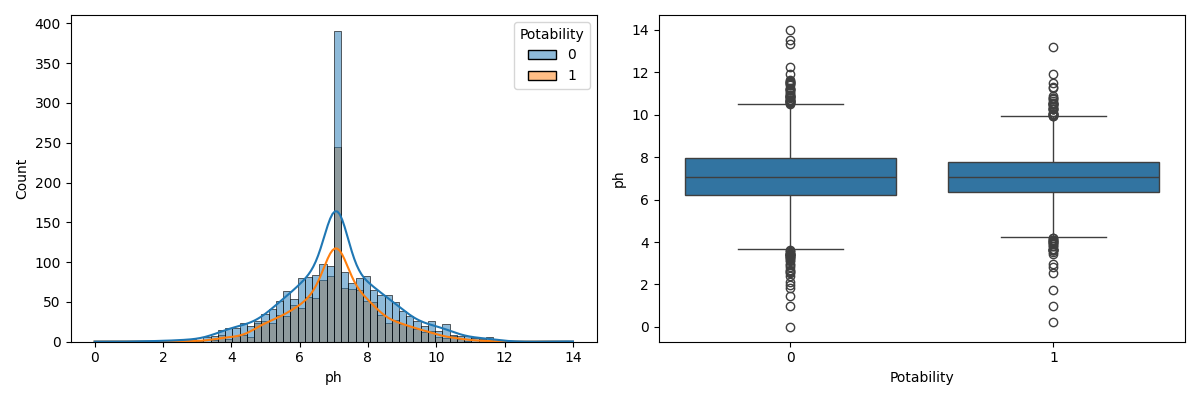
\includegraphics[width=0.9\textwidth]{IMAGE/dist_ph.png}
    \caption{Phân phối và biểu đồ hộp của biến ph sau khi điền khuyết}
\end{figure}

\textbf{Nhận xét:} Biểu đồ cho thấy pH có phân phối chuẩn, tập trung mạnh quanh giá trị trung bình $7.0$. Đỉnh nhọn tại vị trí $7.08$ chính là kết quả của việc điền $491$ dòng dữ liệu thiếu.

\paragraph{Biến "Sulfate":} \leavevmode\\
\begin{figure}[H]
    \centering
    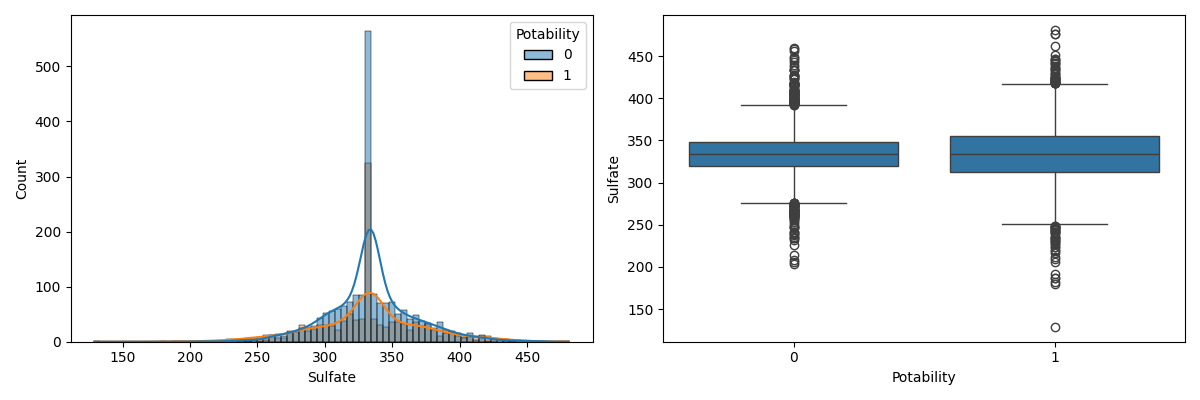
\includegraphics[width=0.9\textwidth]{IMAGE/dist_Sulfate.png}
    \caption{Phân phối của biến Sulfate sau tiền xử lý}
\end{figure}

\textbf{Nhận xét:} Giá trị Sulfate tập trung chủ yếu trong biên độ $[250-450]$ mg/L. Biểu đồ xác nhận việc điền khuyết $781$ dòng bằng giá trị $333.77$ đã được thực thi chính xác.

\paragraph{Biến "Hardness" (Độ cứng):} \leavevmode\\
\begin{figure}[H]
    \centering
    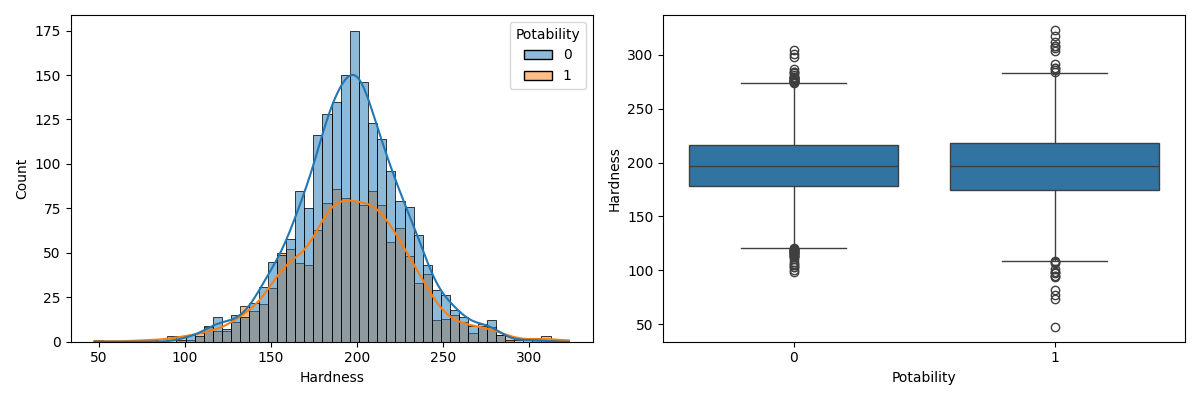
\includegraphics[width=0.9\textwidth]{IMAGE/dist_Hardness.png}
    \caption{Phân phối và biểu đồ hộp của biến Hardness}
\end{figure}
\textbf{Nhận xét:} Biểu đồ mang giá trị phân phối chuẩn ổn định trong biên độ $[100-250]$. Đây là cơ sở để nhóm thực hiện phân loại vào bảng \textbf{Dim\_Hardness}.

\paragraph{Biến "Solids" (Tổng chất rắn hòa tan):} \leavevmode\\
\begin{figure}[H]
    \centering
    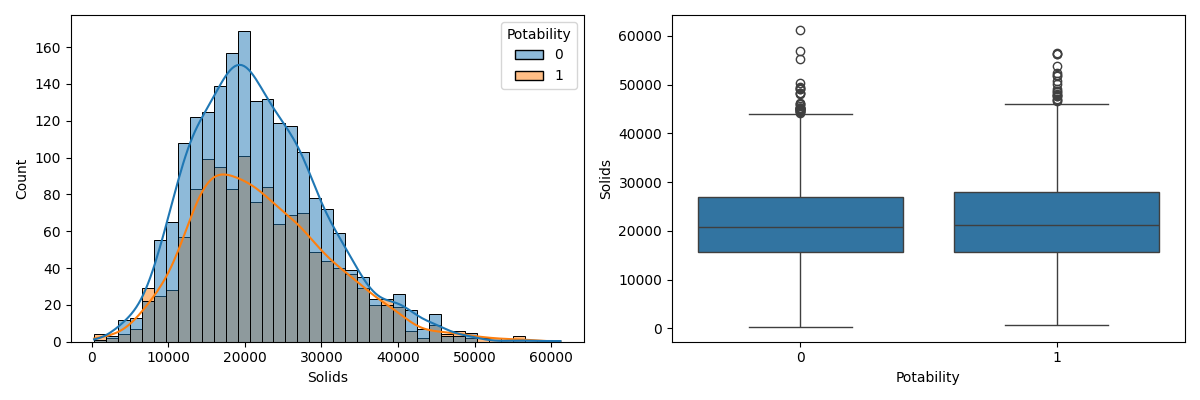
\includegraphics[width=0.9\textwidth]{IMAGE/dist_Solids.png}
    \caption{Phân phối và biểu đồ hộp của biến Solids}
\end{figure}

\textbf{Nhận xét:} Nồng độ Solids có phân phối lệch phải rõ rệt, tập trung trong khoảng $[15,000 - 30,000]$ ppm. Biểu đồ Boxplot xuất hiện nhiều giá trị ngoại lai vượt mức $50,000$ ppm.